\chapter{Literature review}
\label{chapter:literature_review} 


\section{Introduction}


Pneumonia is responsible for approximately 18\% of deaths in children under the age of five (see figure~\ref{pneumonia_stats}). More than 95\% of the childhood pneumonia cases and 99\% of subsequent deaths occur in low and middle income countries (LMIC)\cite{rudan2013epidemiology}.  However, only 3\% of global infectious disease research spending is currently allocated to pneumonia \cite{savethechildren}, such studies being very rare in LMICs due to their resource-intensiveness.

\begin{figure}
	\centering
    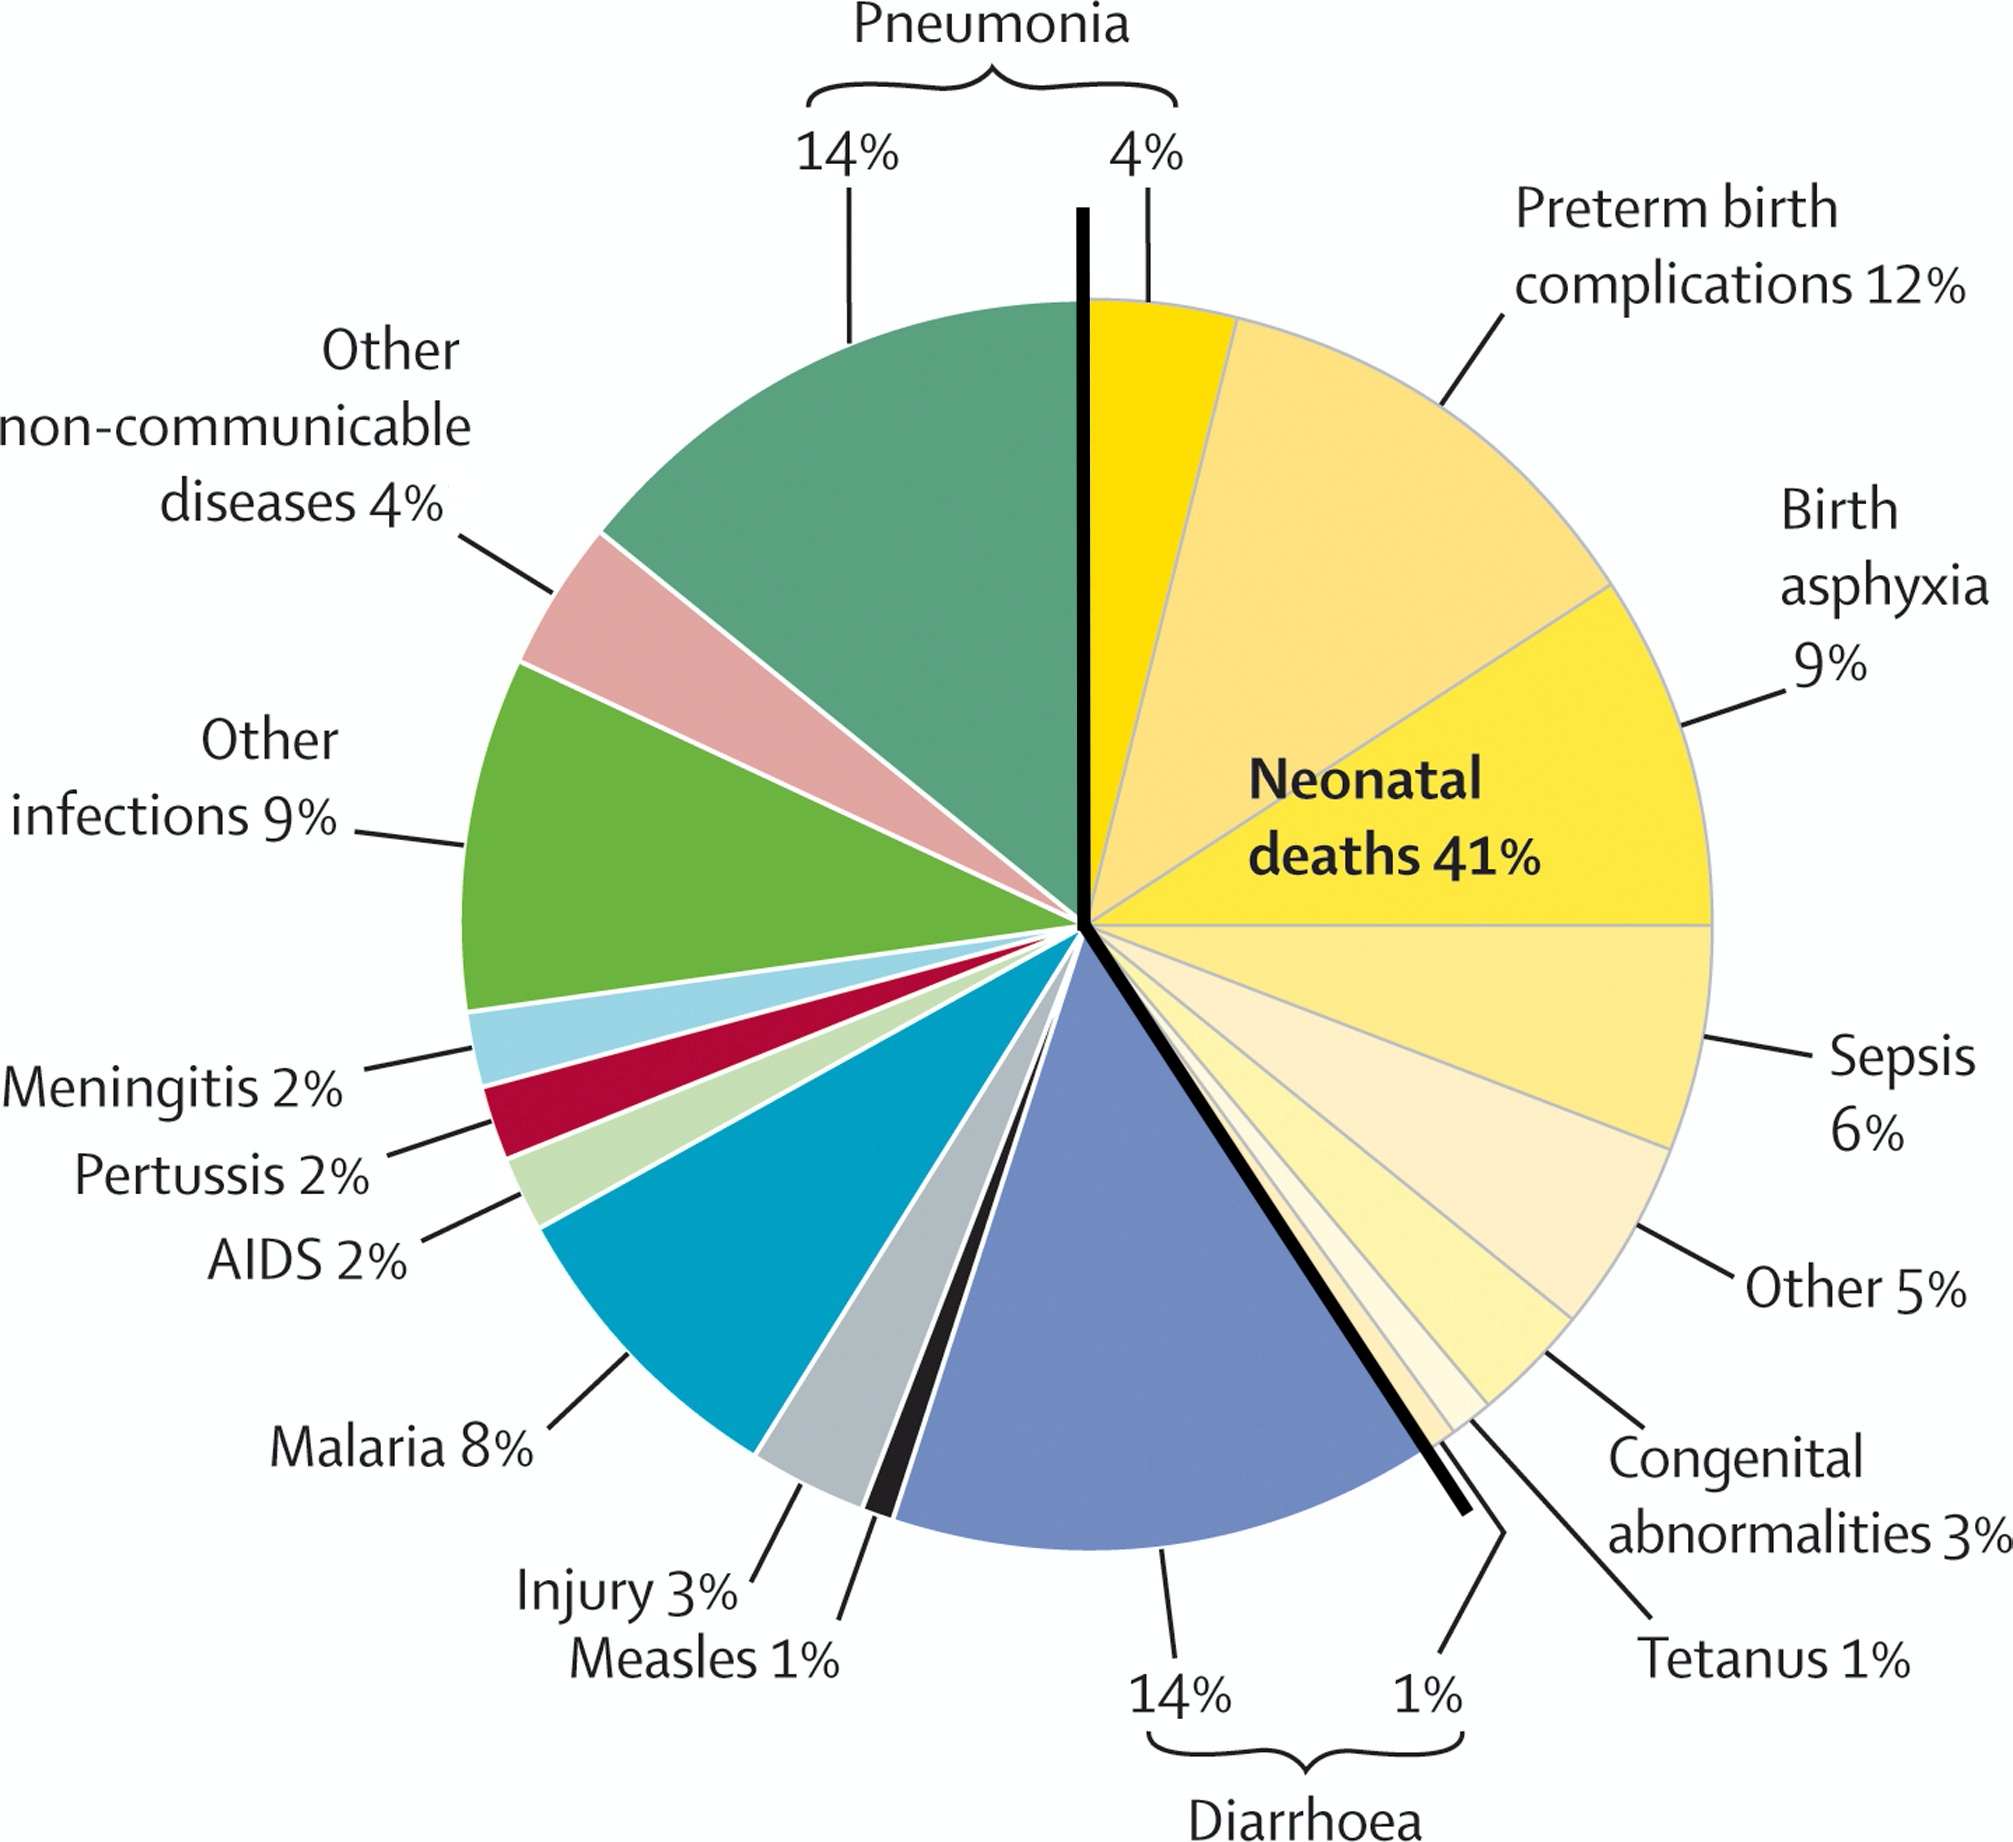
\includegraphics[width=0.7\linewidth,keepaspectratio=true]{pneumonia_stats}
    \caption[Global causes of childhood deaths.] 
    {
    Global causes of childhood deaths. Yellow colour represents deaths of neonates aged 0 – 27 days and the rest correspond to children aged 1 month to 5 years \cite{black2010global}.
    }
    \label{pneumonia_stats}
\end{figure}

Accurate and timely diagnosis of pneumonia is essential for the prevention of hospitalisation and reduction of mortality rates however, access to high-quality healthcare is often limited in LMICs. Appropriate diagnostic assessment of childhood pneumonia typically relies on the use of advanced tools (such as X-rays and blood culture) by a clinical expert who assesses and interprets a combination of clinical measurements \cite{graham2008challenges}. This chapter reviews existing diagnostic innovations for childhood pneumonia. These approaches include image based technologies that can accurately identify abnormal breathing patterns and data-driven machine learning algorithms for interpretation of symptoms. 

\section{Diagnostic Innovations}

\subsection{Pulse oximetry}

Pulse oximetry is a lo-cost technology, widely accepted as the standard for detection of hypoxaemia, an often fatal complication of pneumonia. It has been used to reliably measure hypoxaemia, identifying 20–30\% more cases than clinical signs alone \cite{duke2009pulse}.
 Pulse oximeters are devices that non-invasively measure peripheral oxygen saturation \gls{$SpO_{2}$}. They are inexpensive, portable and, with adequate training and supervision, can be reliably used with children at all levels of the health system in low-resource settings, including by lay community health workers at the household level \cite{goodman2019challenges}. Oxygen saturation estimates may lead to detection of changes in patient conditions that could otherwise be missed, such as a lower \gls{$SpO_{2}$}(<95\%) which indicates hypoxia and insufficient oxygen supply to the human body.
Children with hypoxaemic pneumonia therefore need to be identified, admitted to hospital, given supplemental oxygen and be monitored closely. This necessitates a heightened awareness of the prevalence and the risk of hypoxaemia among children presenting to health-care facilities and robust mechanisms to detect it \cite{subhi2009prevalence}.

\subsection{Lung auscultation}

Lung auscultation is the use of a stethoscope to acoustically assess airflow through the trachea-bronchial tree and remains an important component of pneumonia diagnosis, with more predictive accuracy than an initial clinical assessment alone \cite{pervaiz2018building}. 
The addition of lung auscultation as a diagnostic tool improved the classification of radiographically confirmed clinical pneumonia in cases with decreased breath sounds, absence of wheezes, but presence of crackles \cite{pervaiz2018building}. Crackles are discontinuous, explosive, and non musical adventitious lung sounds normally heard in inspiration and sometimes during expiration. Crackles are usually classified as fine or coarse based on their duration, loudness, pitch, timing in the respiratory cycle, and relationship to coughing and changing body position\cite{sarkar2015auscultation}. Although traditional acoustic stethoscopes are inexpensive and portable, the implementation of lung auscultation in low-resource settings is limited by challenges including the training required to recognise the specific signals necessary to make a diagnosis. Computerised analysis of lung sounds has been suggested and explored as a tool for automated classification of acoustic patterns and different respiratory conditions.

\subsection{Other innovations}

Other diagnostic innovations being developed include automated respiratory rate counters with a variety of technologies such as accelerometers and bioimpedance among others). The combination of several diagnostic and prognostic innovations into an integrated instrument could improve identification of pneumonia and its severity \cite{ginsburg2013innovations}. Table~\ref{innovations} summarises some of the recent devices proposed.

\begin{table}
	\centering
	\caption[COMPLETE ME]
	{
	Summary of diagnostic innovations that have been recently developed, or are currently under development in the context of childhood pneumonia. sources (UNICEF 2013) and personal research.
	}
	\begin{tabular}{p{2cm}p{11.5cm}}
	 	\tableHeaderStart 
		Diagnostic Innovation & \multicolumn{1}{c}{\textbf{Description}} \\
	     \tableHeaderEnd
			mPneumonia & An Android mobile application which automates the WHO
			IMCI protocol. The app paired with a software-based breath counter and a 
			pediatric pulse oximeter to facilitate rapid identification of fast breathing 
			\cite{ginsburg2015mpneumonia}. \\        
		\hline
		WHO ARI timer and Counting Beads & Designed as a simple and cheap way to help community health workers count breaths. The counting beads comprise of one strand of beads, non-specific for children ages 0–5 years. The strand is necklace shaped and has a protruding start/end bead. The health worker count breaths by moving a bead for each breath. When 1 minute has passed the \gls{chw} counts back the beads to determine the RR. Counting beads should be  used in conjunction with the ARI Timer. \\  
		\hline
		RRate mobile application & RRate measures RR by recording the time interval in between breaths as the user taps on a touch sensitive screen of a mobile device in time with inspiration.  Once a consistent set of taps has been achieved, a chime noise is played and the result displayed \cite{karlen2014improving}.\\  
	    \hline
	  	Amplified stethoscopes e.g ThinkLabs \& Ekuore & Digital stethoscopes that can transmit lung signals (auscultation) onto a smart phone \cite{naydenova2018machine}. \\  
		\hline
		The HealthPatch  MD & Consists of two ECG  electrodes,  a  tri-axial  accelerometer, micro-controller and  transceiver within a patch that straps like a bandage over the heart. The device measures HR, RR, steps and posture and connects wirelessly to a smartphone via bluetooth \cite{breteler2018reliability}.\\
		\hline
	\end{tabular}
	\label{innovations}
\end{table}


\section{Vital sign acquisition and estimation}

Respiratory rate can be difficult to measure in a standardised way. It is typically counted manually in low-resource settings, using timers or counting beads. Manual measurement, although often the reference standard, can be imprecise and is affected by intra-observer variation as it requires focused concentration. It is often required to be measured from a crying, irritable and moving child. Automated devices to compute RR are more commonly available in well-resourced settings. These include extracting respiration from the photoplethysmography (PPG) signal from a pulse oximeter, or remotely using a modern camera.

\subsection{Pulse oximetry}

One of the earliest light-based continuous vital-sign monitoring methods developed was pulse oxmetry, first explored in the 1930s \cite{elgendi2019use}. Pulse oximetry is a non-invasive technology that uses a light source and a photo detector at the surface of skin to measure the volumetric variations of blood circulation. 
The light source illuminates the tissue, and the photo detector measures the small variations in the reflected or transmitted light intensity associated with changes in perfusion. The fundamental principle of pulse oximetry relies on the differences in arbsorption of blood and other tissue components at different wavelengths\cite{ugnell1995time}.
When the heart pumps blood to the body and the lungs during systole, the amount of blood that reaches the capillaries in the skin surface increases, resulting in more light absorption. The blood then travels back to the heart through the venous network, leading to a decrease of blood volume in the capillaries and less light absorption\cite{sun2015photoplethysmography}. These changes can be recorded as the PPG waveform, comprising a pulsatile signal from which oxygen saturation (\gls{$SpO_{2}$}) and other vital signs such as heart rate (\gls{hr})and respiratory rate (\gls{rr}) can be computed.

\begin{figure}
  \centering
    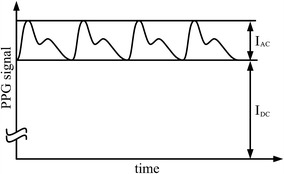
\includegraphics[width=0.5\linewidth,keepaspectratio=true]{PPG_signal.png}
    \caption[A typical PPG waveform]
    {
    A typical PPG waveform showing the AC component and DC component \cite{guo2015reflective}
    }    
    \label{ppgsignal}
\end{figure}

The pulsatile changes of the \gls{ppg} waveform is often called the "AC" component, it is synchronous with the beating heart. In contrast, the non-pulsating component "\gls{dc}" is a function of the basic blood volume,  respiration,  the  sympathetic nervous system, and thermo-regulation. As shown  schematically  in figure \ref{ppgsignal},  most of the signal is static (DC) and represents the light that has not been modulated by arterial blood \cite{mendelson1992pulse}. 

\subsection{Wearable technology}

There is a growing interest in continuous monitoring of vital signs outside of traditional settings such as the clinic or hospital. The development of wearable technology that unobtrusively and reliably monitors vital signs has allowed the evaluation of patient recovery after discharge and the monitoring of those deemed at risk or suffering from chronic illness \cite{bonato2005advances}. Wearable devices can incorporate a range of sensors such as PPG, accelerometer and gyroscopes. These devices can be worn in a variety of different locations, including finger, ear lobe and wrist to provide measurements from these sensors.

\subsection{PPG imaging}

Despite conventional PPG’s wide range of applications, there are several significant limitations to the usefulness. Current monitoring systems available to track changes in the vital signs of patients require contact with the subject by using adhesive electrodes or sensors \cite{villarroel2017non}. These can however damage the fragile skin of young infants or cause stress and discomfort. The introduction of fast digital cameras into clinical imaging monitoring and diagnosis systems, the desire to reduce the physical restrictions, and the possible new insights that might come from perfusion imaging and mapping inspired the evolution of conventional PPG technology to photoplethysmographic imaging (PPGi) \cite{sun2015photoplethysmography}. Video-based vital sign monitoring extends the concepts of traditional PPG, using the multiple photosites present in an imaging sensor to record the blood volume changes associated with the cardiac cycle. These physiological changes result in a signal from which vital signs such as HR, RR, oxygen saturation \gls{$SpO_{2}$} and others can be estimated \cite{tarassenko2014non, villarroel2014continuous}.

In 2008,  Verkruysse \textit{et al }\cite{verkruysse2008remote} showed for the first time, that PPG signals could be remotely acquired from the human face with a simple, digital, consumer-level camera as the detector more than 1 m away. The study conducted used daylight as the illumination source in combination with normal artificial fluorescent light. Regions of interest (ROIs) were selected in images of the faces from human volunteers. 
The authors presented evidence that the reflectance signals were pulsatile cardiac signals by showing that signals corresponding to movement of facial areas with no exposed skin (edge of the face and hair above the ear) were not predominantly at the heart rate frequency. The green channel was found to provide the strongest plethysmographic signal amplitude, corresponding to an absorption peak by oxyhaemoglobin, but the red and blue channels were also shown to contain plethysmographic information. The paper showed how heart rate could be extracted from the frequency content of these images using the fast Fourier transform (FFT) for 10s windows, and hinted at how respiratory rate might be computed using an \gls{roi} which encompasses the entire face.

In 2010, Tan \textit{et al} presented a real-time vision based respiration monitoring system. The method involved image and signal processing techniques to extract chest and abdominal movement information from a sequence of video images recorded using a single video camera. The system provided a real-time respiration signal from which RR was computed \cite{tan2010real}. In the same year, Bai \textit{et al}\cite{bai2010design} designed an embedded monitoring system for body breath detection using a webcam. 
Their design employed a temporal differencing algorithm, which subtracts subsequent frames to detect moving objects \cite{lien2008monitoring}. This was used to identify chest movement and determine the respiratory rate. The developed system estimated the respiration rate of sleeping or stationary subjects with a static background, which poses a limitation for monitoring children or infants.

Jorge \textit{et al} proposed a new method for use in neonates in 2017, which was incorporated into a Cessation Of Breathing Events (COBE) detection system. For this method, skin pixels were identified first in each frame using a skin classifier and the ROI for motion analysis selected. Motion analysis was done to detect breathing movements and estimate their frequency. A binary signal quality index (SQI) was produced for these estimates based on the level of activity on the video sequence. In contrast to the previous methods discussed, this approach is able to account for subject motion and changes in background lighting \cite{jorge2017non}.

\section{Respiratory signal processing}

\subsection{Respiratory signal extraction }

Extracting a respiratory signal from \gls{ppg} requires the identification of respiratory modulation components driven by the fluctuation of blood volume in the peripheral vascular bed. These modulation components are pulse amplitude, baseline and respiratory sinus arrhythmia (RSA).

\begin{figure}
  \centering
    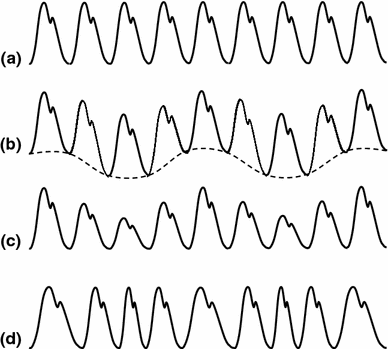
\includegraphics[width=0.5\linewidth,keepaspectratio=true]{nicu_modulation.png}
    \caption[Modulation of the PPG signal due to respiration.]
    {
    Modulation of the PPG signal due to respiration; a) Unmodulated PPG showing cardiac pulse waveforms; b) Baseline modulation (cardiac pulses riding on top of baseline shown dashed); c) Amplitude modulation (cardiac pulse amplitudes varying over the respiratory cycle); d) RSA (pulse period varying over the respiratory cycle). Figure reproduced from \cite{addison2012developing}.
    }
	\label{modulation)}
\end{figure}

\begin{itemize}

	\item \textbf{Baseline modulation:} A baseline modulation of the PPG signal is caused by changes in venous return secondary to changes in intra-thoracic pressure throughout the respiratory cycle. During inspiration, decreases in intra-thoracic pressure result in a small decrease in central venous pressure increasing venous return. The opposite occurs during expiration. As more blood is averted from the low pressure venous system and the venous bed cyclically fills and drains, the baseline PPG is modulated accordingly \cite{addison2012developing}. This effect is shown in figure~\ref{modulation)}b.
	
	\item \textbf{Amplitude modulation:} Amplitude modulation is caused directly by changes in intra-thoracic pressure during the respiratory cycle. These changes result in respiratory oscillations in the amplitude of the signal, and this effect is shown in figure~\ref{modulation)}c.
	
	\item \textbf{RSA}: Respiratory sinus arrhythmia is a variation in heart rate that occurs throughout the respiratory cycle. It is well documented that heart rate increases during inspiration and decreases during expiration. While the precise mechanisms of RSA remain disputed, it is a result of autonomic nervous system activity fluctuation during respiration. This effect is shown in figure~\ref{modulation)}d.

\end{itemize}

The extraction of respiratory components is particularly challenging as the three aforementioned respiratory modulations may be present to varying degrees across the patient population. A further challenge for algorithms to extract respiratory signals is that respiratory components often appear concurrently with a range of other low frequency artefacts due, for example, to voluntary or involuntary movements of the patients or blood pressure changes \cite{addison2012developing}. Appropriate signal processing techniques must therefore be implemented to accurately extract this information.

\subsection{Signal processing techniques }

From the presence of the respiratory response in a PPG waveform, many researchers have been motivated to develop or utilise methods for RR estimation, such as digital filters, auto-regressive (AR) models, variable frequency complex demodulation and particle filters.

\subsubsection{Digital filtering}

In their 2000 study, Nilsson \textit{et al} \cite{nilsson2000monitoring} extracted the respiratory synchronous part of the PPG signal using a band pass filter. A 3$^{rd}$ order Butterworth band-pass filter with a pass-band from \textit{f} = 0.1 – 0.3 Hz (6 to 18 breaths/min) was used. Detection of breaths in the filtered PPG signals was done both visually and by using an automated algorithm. In 2009, Nakajima et al. developed a technique that used digital filters to estimate HR and RR from a PPG signal. The cut-off frequency of the respiratory signal filter was selected automatically depending on the heart rate so that a higher cut-off frequency was used at higher heart rates \cite{nakajima1996monitoring}. Despite the complexity of the algorithm, it did not perform as well as the method proposed by Nilsson \textit{et al}, and had an average error of over 3 breaths per minute when compared to the reference rate. 

\subsubsection{Auto-regressive modelling}

Auto-regressive (AR) modelling looks for regular frequencies in a signal which is deemed to be stationary over the period of analysis. It models this periodic behaviour by comparing the signal with its own past values at various time lags \cite{takalo2005tutorial}. In 2007, Fleming and Tarassenko developed a method to estimate RR from a PPG signal using an AR model. This method was shown to perform better than both the digital filtering and wavelet decomposition methods \cite{fleming2007comparison}. An AR method involving factorising the estimated AR parameters into multiple pole terms was later presented by Lee \textit{et al} \cite{lee2010respiratory}. The pole with the highest magnitude was chosen to represent the respiratory rate. The method showed accurate respiratory rate extraction, especially for high respiratory rates (36 – 48 breaths/min). To mitigate a previously described limitation of AR models, particle filtering was introduced to track moving targets. Recent efforts have been made to develop efficient algorithms for real-time implementation \cite{hong2007design}. 

HR and RR estimation using AR modelling has also been proposed for video-based vital sign monitoring by Tarassenko \textit{et al.} \cite{tarassenko2014non}. This method also cancels out aliased frequency components caused by artificial light flicker using AR modelling and pole cancellation.
